\documentclass[11pt]{article}

\usepackage{fullpage}
\usepackage{graphicx}
\usepackage{amsmath}
\usepackage{amssymb}
\usepackage{amsthm}
\usepackage{fancyvrb}

\parindent0in
\pagestyle{plain}
\thispagestyle{plain}

\newcommand{\myname}{Mehshan Mustafa}
\newcommand{\dated}{\today}

\newenvironment{theorem}[2][Theorem]{\begin{trivlist}
\item[\hskip \labelsep {\bfseries #1}\hskip \labelsep {\bfseries #2.}]}{\end{trivlist}}
\newenvironment{lemma}[2][Lemma]{\begin{trivlist}
\item[\hskip \labelsep {\bfseries #1}\hskip \labelsep {\bfseries #2.}]}{\end{trivlist}}
\newenvironment{exercise}[2][Exercise]{\begin{trivlist}
\item[\hskip \labelsep {\bfseries #1}\hskip \labelsep {\bfseries #2.}]}{\end{trivlist}}
\newenvironment{problem}[2][Problem]{\begin{trivlist}
\item[\hskip \labelsep {\bfseries #1}\hskip \labelsep {\bfseries #2.}]}{\end{trivlist}}
\newenvironment{question}[2][Question]{\begin{trivlist}
\item[\hskip \labelsep {\bfseries #1}\hskip \labelsep {\bfseries #2.}]}{\end{trivlist}}
\newenvironment{corollary}[2][Corollary]{\begin{trivlist}
\item[\hskip \labelsep {\bfseries #1}\hskip \labelsep {\bfseries #2.}]}{\end{trivlist}}
\newenvironment{solution}{\begin{proof}[Solution]}{\end{proof}}
\newenvironment{idea}[2][Proof Idea.]{\textit{#1} #2}

\begin{document}

\textbf{Introduction to the Theory of
Computation}\hfill\textbf{\myname}\\[0.01in]
\textbf{Chapter 1: Reqular Languages}\hfill\textbf{\dated}\\
\smallskip\hrule\bigskip

\begin{problem}{1.31}
For any string $w = w_{1} w_{2} \cdots w_{n}$, the reverse of $w$, written $w^{R}$ , is the string {w} in reverse order, $w_{n} \cdots w_{1} w_{2}$. For any language $A$, let $A^{R} = \lbrace w^{R} \, | \, w \, \epsilon \, A \rbrace$. Show that if $A$ is regular, so is $A^{R}$.
\end{problem}

\begin{idea}
If A is regular, then there exists a DFA, say $N$ that recognizes it. Take $N$ and construct a new NFA $N'$ to recognize $A^{R}$. $N'$ has all the states of $N$, but the transitions are reversed. Start state of $N$ is the accept state of $N'$ has a new start state, say $q_{s}$ with $\epsilon$ transitions to every accept state in $N$.
\end{idea}

\begin{center}
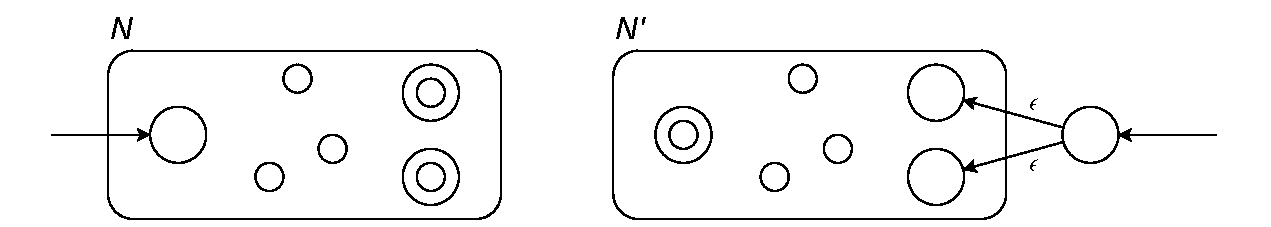
\includegraphics[scale=0.7]{Figures/Problem1.31.pdf} \\
When $N$ computes on some $w \, \epsilon \, A$, it starts at the accept state, tranisitions through some intermediate states and finally stops at some accept state, whereas $N'$ starts simultaneously from all the accept states of $N$ and transitions backwards to reach the start state of $N$, which is the only accept state in $N'$.
\end{center}

\begin{proof}
The proof is by construction. Let $N = (Q, \Sigma, \delta, q_{0}, F)$ be the DFA that recognizes $A$. Construct $N' = (Q', \Sigma, \delta', q_{0}', F')$ to recognize $A^{R}$:
\begin{enumerate}
\item $Q' = Q \cup \lbrace q_{s} \rbrace$
\item $q_{s}$ is the start state
\item $F' = \lbrace q_{0} \rbrace$
\item Define $\delta'$(q, a) so that for any $q \, \epsilon \, Q'$ and any $a \,  \epsilon \, \Sigma_{\epsilon}$:
\end{enumerate}
\begin{center}
$\displaystyle \delta '( q,\ a) \ =\begin{cases}
F & q=q_{s} \ and\ a\ =\ \epsilon \\
\phi  & q=q_{s} \ and\ a\ \neq \ \epsilon \\
\{q'\ |\ q'\ \epsilon \ Q\ and\ \delta ( q',\ a) \ =\ q\} & q\ \epsilon \ Q
\end{cases} \ \ $
\end{center}
\end{proof}

\end{document}